\subsection{FEMTO-ST}

\begin{frame}{FEMTO-ST}
    \begin{block}{Franche-Comté Electronique Mécanique Thermique et Optique - Sciences et Technologies}
        % \begin{itemize}
        %     \item Unité mixte de recherche associée au CNRS et rattachée simultanément à : UMLP, Supmlcrotech, UTBM
        %     \item Créer le $1^{er}$ janvier 2004 par la fusion de 5 laboratoires de Franche-Comté. $1^{er}$ janvier 2012 incorpore le laboratoire d'informatique de l'UMLP.
        %     \item Plus de 700 membres, plus gros institut de recherche dans les sciences pour l'ingénieur en France
        %     \item Répartie sur Besançon, Belfort et Montbéliard
        % \end{itemize}
        \begin{itemize}
            \item Statut : unité mixte de recherche du CNRS, rattachée à l'UMLP, Supmicrotech et l'UTBM.
            \item Création : fusion de cinq laboratoires en 2004, puis intégration du laboratoire d'informatique de l'UMLP en 2012.
            \item Effectif : plus de 700 membres, premier institut français de recherche en sciences pour l'ingénieur.
            \item Implantation : Besançon, Belfort et Montbéliard.
        \end{itemize}
    \end{block}
\end{frame}

\subsection{DISC}

\begin{frame}{DISC}
    \begin{block}{Département d'Informatique et Systèmes Complexes}
    % \begin{itemize}
    %     \item Département de FEMTO-ST qui traite des sciences informatique
    %     \item Objectif principal des recherches menées est de modéliser, simuler, développer et valider les systèmes complexes
    %     \item Compte environ 100 personnes, répartis en 4 équipes de recherche :
    %     \begin{itemize}
    %         \item Algorithmique Numérique Distribuée (AND)
    %         \item Design, Evaluation and Optimisation of Distributed and Intelligent Systems (DEODIS)
    %         \item Optimisation, Mobility, NetworkIng (OMNI)
    %         \item Verification et validation de logiciels et de systèmes embarqués (\textbf{VESONTIO})
    %     \end{itemize}
    % \end{itemize}
    
    \begin{itemize}
        \item Domaine : département de FEMTO-ST dédié aux sciences informatiques.
        \item Objectif : modéliser, simuler, développer et valider des systèmes complexes.
        \item Composition : environ 100 membres répartis en quatre équipes de recherche :
        \begin{itemize}
            \item Algorithmique Numérique Distribuée (AND)
            \item Design, Evaluation and Optimisation of Distributed and Intelligent Systems (DEODIS)
            \item Optimisation, Mobility, NetworkIng (OMNI)
            \item Verification et validation de logiciels et de systèmes embarqués (\textbf{VESONTIO})
        \end{itemize}
    \end{itemize}
    \end{block}
\end{frame}

\subsection{Projet ADAPT}

\begin{frame}{Mise en contexte}
    \begin{block}{Nécessité}
        \begin{itemize}
            \item Systèmes à composants de plus en plus complexes.
            \item Outils évolutifs.
            \item Adaptation aux besoins des utilisateurs et de la recherche.
        \end{itemize}
    \end{block}
\end{frame}

\begin{frame}{ADAPT : Adaptation dynamique de systèmes à composants hiérarchiques}

\vspace{5mm}

\begin{block}{Détails}
\begin{itemize}
    \item Projet ANR.
    \item 48 mois (commencé en mars 2024).
    \item INRIA (Lille), FEMTO-ST, Verimag (Grenoble).
\end{itemize}
\end{block}

\begin{block}{Objectif principal}
    Développer un cadre formel et des outils permettant de concevoir des systèmes cyber-physiques adaptatifs de manière correcte par construction.
\end{block}

\begin{block}{}
    Il s'intéresse en particulier aux systèmes composés d'un grand nombre de composants modulaires, comme les robots modulaires Blinky Blocks, capables de se reconfigurer dynamiquement pour accomplir une tâche commune.
\end{block}
    
\end{frame}

\begin{frame}{Objectifs scientifiques}

\begin{block}{Objectifs}
    % \begin{itemize}
    %     \item Etendre les modèles à composants hiérarchiques afin de permettre la description de systèmes complexes composés de nombreux modules
    %     \item Intégrer des mécanismes de contrôle adaptatif directement dans ces modèles
    %     \item Implémenter ces mécanismes d'adaptation dans une infrastructure de modélisation fondée sur les systèmes à composants
    %     \item Valider les mécanismes proposés par simulation avant leur déploiement
    % \end{itemize}
    
    \begin{itemize}
        \item Étendre les modèles à composants hiérarchiques.
        \item Intégrer le contrôle adaptatif.
        \item Implémenter les mécanismes d'adaptation.
        \item Valider les mécanismes par simulation.
    \end{itemize}
\end{block}

\begin{block}{}
    Développement de CHIPS (Control of Hierarchical Interconnected Programmable Systems) qui permet de décrire des systèmes hiérarchiques composés de composants modulaires.
\end{block}
    
\end{frame}

\begin{frame}{Schéma de la chaîne de compilation}
\begin{figure}
    \centering
    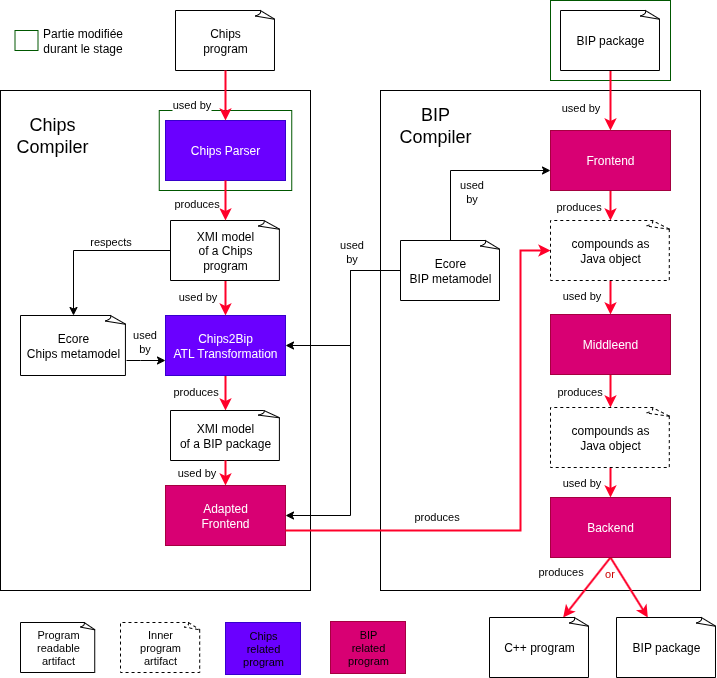
\includegraphics[width=0.5\textwidth]{img/architecture_partie_modifier.png}
\end{figure}
\end{frame}

\begin{frame}{Objectifs du stage}
\begin{block}{Objectifs}
\begin{itemize}
    \item Migrer le parseur historique vers ANTLR4 afin d'obtenir une architecture plus robuste et plus facilement extensible.
    \item Adapter le générateur XMI au nouvel arbre syntaxique produit par ANTLR4.
    \item Développer une bibliothèque de filtres numériques.
    \item Implémenter plusieurs mécanismes d'anti-windup destinés aux contrôleurs PID.
    \item Intégrer l'ensemble de ces composants à la chaîne de compilation CHIPS.
\end{itemize}
\end{block}
    
\end{frame}